\subsection{ソフトウェアアーキテクチャ記述}

\subsubsection*{アーキテクチャ記述の役割}
\addcontentsline{toc}{subsubsection}{アーキテクチャ記述の役割}
小さなシステムを一人で作る場合、アーキテクチャは頭の中にあるだけでも作業できることがある。しかし、大規模で複雑なシステムをチームで作り、運用し、保守する場合には、頭の中の理解だけでは不十分である。人が入れ替わり、要求が変わり、構成が進化するため、アーキテクチャを具体的な成果物として残す必要がある。

この成果物を\keyterm{アーキテクチャ記述}\en{architecture description}という。アーキテクチャ記述は、開発者にとっては構築の設計図であり、テスト担当、品質保証担当、認証担当、運用担当、保守担当にとっては、自分の作業を進めるための根拠である。

かつては、アーキテクチャ記述は文章と非形式的な図で行われることが多かった。しかし、利害関係者と関心事が多様になるにつれて、単一の図ですべてを表すことは難しくなった。そのため、目的や読者に応じて複数のビューを使う方法が重要になった。

\subsubsection{アーキテクチャビューとビューポイント}
\keyterm{ビュー}\en{architecture view}とは、アーキテクチャの一面を表すものである。たとえば、機能要求をどう満たすかを示す論理ビュー、並行処理や実行時相互作用を示すプロセスビュー、システムをどこに配置するかを示す物理ビュー、実装単位や依存関係を示す開発ビューがある。

ビューを分ける理由は、関心事を分離するためである。性能を確認したい人、安全性を確認したい人、配置を考える人、コード分担を考える人は、それぞれ必要な情報が違う。一つの図にすべてを詰め込むと、誰にとっても読みにくい図になる。

\keyterm{ビューポイント}\en{architecture viewpoint}とは、ビューを作成し、解釈し、利用するための規約である。どの要素を使うか、どの関係を描くか、どの記法を使うか、どの関心事に答えるか、誰が読むかを定める。ビューポイントは、ビューの「描き方の型」である。

\par\smallskip\noindent\refstepcounter{table}\label{tab:ch02-03}\textbf{表 \thetable: 第02章 ソフトウェアアーキテクチャ 表03}\par\smallskip
\begin{longtable}{P{0.25\linewidth}P{0.67\linewidth}}
\toprule
種類 & 説明 \\
\midrule
モジュールビューポイント & 実装単位としてのモジュール、その責任、依存関係、分割を表す。 \\
構成要素・接続子ビューポイント & 実行時の大きな構成要素と、それらをつなぐ通信・接続関係を表す。 \\
論理ビューポイント & 対象領域の主要概念、能力、関係を表す。 \\
シナリオ・ユースケースビューポイント & 利用者がシステムとどのように相互作用するかを表す。 \\
情報ビューポイント & 重要な情報、データの保管、アクセス、流れを表す。 \\
配置ビューポイント & ソフトウェアをどの実行環境、機器、ネットワークに置くかを表す。 \\
\bottomrule
\end{longtable}

複数のビューを使うと、別の問題が生じる。ビュー同士が矛盾する可能性である。たとえば、開発ビューでは存在する構成要素が配置ビューにはない、または論理ビューの関係が実行時ビューで説明されていない、といった問題である。これを複数ビュー問題という。対策として、ビュー間の対応関係、追跡可能性、整合性規則を明示する必要がある。

ビューを構成する方法には二つの代表的な考え方がある。\keyterm{合成的手法}では、複数のビューを別々に作り、対応規則で統合する。\keyterm{射影的手法}では、一つの統一モデルから複数のビューを取り出す。射影的手法は整合性を保ちやすいが、統一モデルが表せない関心事には弱い。

\begin{figure}[htbp]
\centering
\IfFileExists{assets/generated_figures/ch02/fig-ch02-04.png}{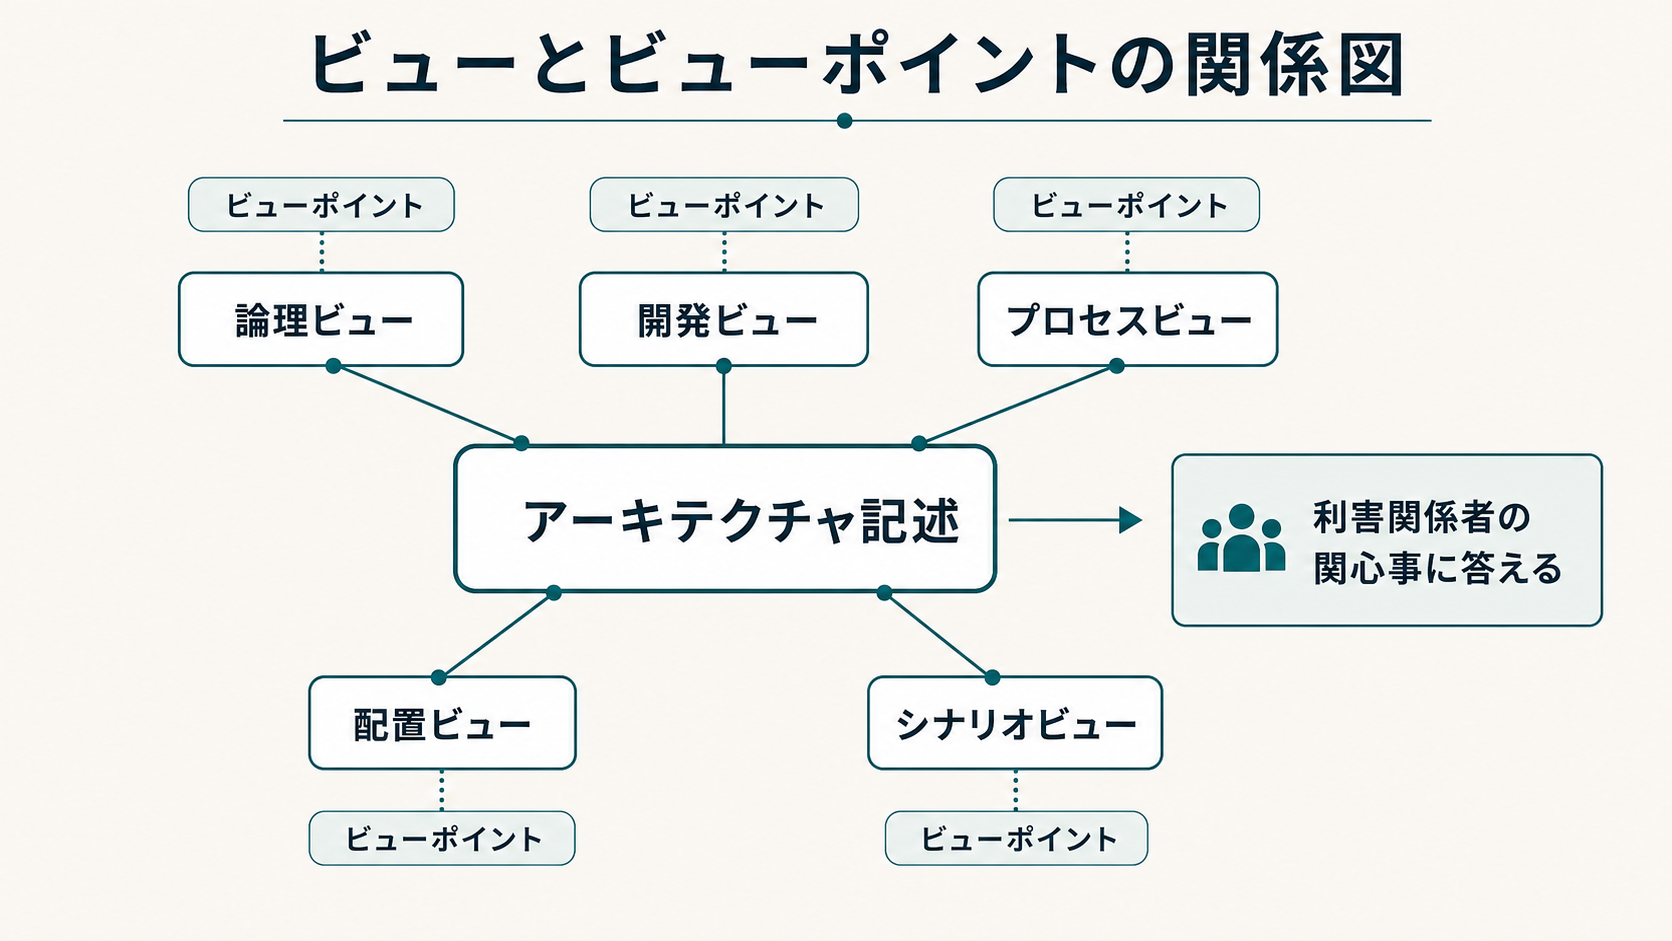
\includegraphics[width=0.96\linewidth]{assets/generated_figures/ch02/fig-ch02-04.png}}{\fbox{\parbox[c][48mm][c]{0.9\linewidth}{\centering 画像生成待ち\\ビューとビューポイントの関係図}}}
\caption{ビューとビューポイントの関係図}
\label{fig:ch02-04}
\end{figure}

\subsubsection{アーキテクチャパターン、様式、参照アーキテクチャ}
\keyterm{アーキテクチャ様式}\en{architectural style}とは、ソフトウェアシステムを構成する特定の作り方であり、システム全体または大きな部分に特徴を与える。たとえば、層化様式、パイプ・アンド・フィルタ、クライアントサーバ、n 層構成、マイクロサービスなどがある。

\keyterm{アーキテクチャパターン}\en{architectural pattern}とは、ソフトウェアシステムの文脈で繰り返し現れる問題に対する共通の解決法である。様式がシステム全体の大きな構成傾向を表しやすいのに対し、パターンは特定の問題への再利用可能な解決法として理解しやすい。ただし、両者の境界は厳密ではない。様式をパターンとして表すこともある。

\par\smallskip\noindent\refstepcounter{table}\label{tab:ch02-04}\textbf{表 \thetable: 第02章 ソフトウェアアーキテクチャ 表04}\par\smallskip
\begin{longtable}{P{0.28\linewidth}P{0.30\linewidth}P{0.30\linewidth}}
\toprule
分類 & 例 & 初学者向けの理解 \\
\midrule
一般的な構造 & 層化、呼出し復帰、パイプ・アンド・フィルタ、黒板、サービス、マイクロサービス & 大きな構成の型である。 \\
分散システム & クライアントサーバ、n 層、ブローカ、発行購読、REST & ネットワーク越しの構成や通信の型である。 \\
方法に基づく構造 & オブジェクト指向、イベント駆動、データフロー & 設計や処理の考え方に基づく型である。 \\
利用者相互作用 & モデル・ビュー・コントローラ、表示・抽象・制御 & 画面や操作の分離に関する型である。 \\
適応システム & マイクロカーネル、反射、メタレベルアーキテクチャ & 変化や拡張に対応しやすくする型である。 \\
\bottomrule
\end{longtable}

\keyterm{参照アーキテクチャ}\en{reference architecture}とは、他のアーキテクチャを導く、または制約するアーキテクチャである。個別システム、製品系列、特定領域のシステムを作るときの共通基盤になる。自動車、医療、モノのインターネット、クラウド、航空電子、製造、通信などの領域で使われる。

\begin{statementbox}{区別の目安}
様式は「全体としてどのような形で作るか」、パターンは「繰り返す問題にどう答えるか」、参照アーキテクチャは「ある領域で個別アーキテクチャを作るための基準」である。
\end{statementbox}

\begin{figure}[htbp]
\centering
\IfFileExists{assets/generated_figures/ch02/fig-ch02-05.png}{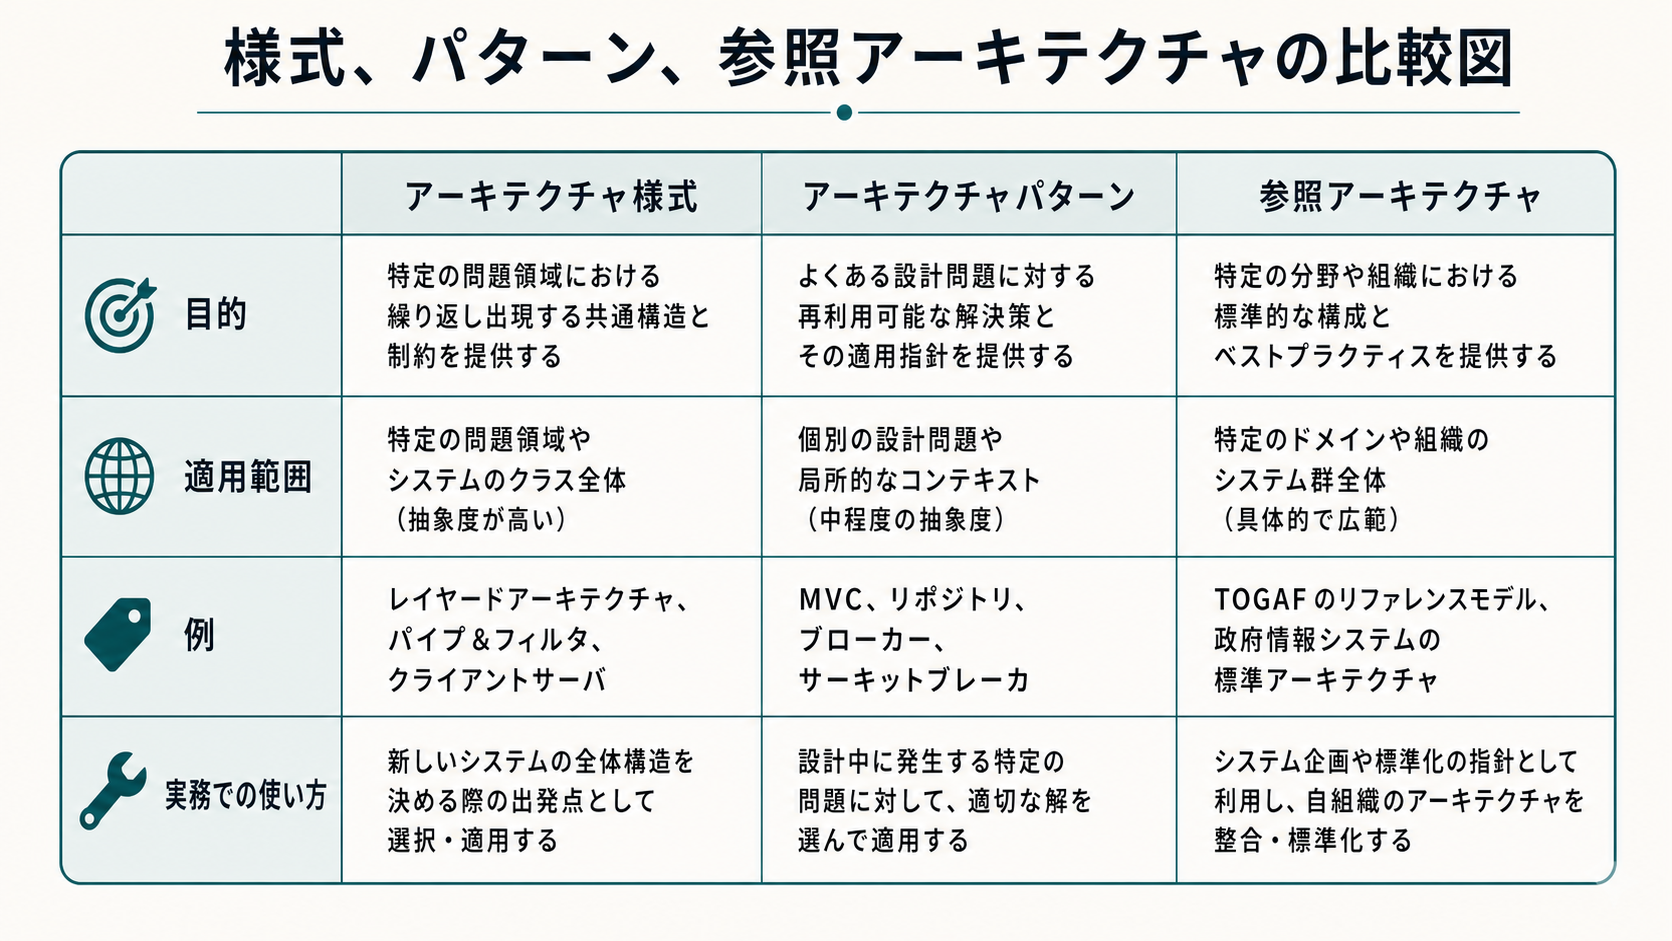
\includegraphics[width=0.96\linewidth]{assets/generated_figures/ch02/fig-ch02-05.png}}{\fbox{\parbox[c][48mm][c]{0.9\linewidth}{\centering 画像生成待ち\\様式、パターン、参照アーキテクチャの比較図}}}
\caption{様式、パターン、参照アーキテクチャの比較図}
\label{fig:ch02-05}
\end{figure}

\subsubsection{アーキテクチャ記述言語とアーキテクチャ枠組み}
\keyterm{アーキテクチャ記述言語}\en{Architecture Description Language, ADL}とは、ソフトウェアアーキテクチャを表すための領域特化言語である。ADL は、もともと大規模プログラミングにおけるモジュール相互接続言語から発展した。特定の領域や様式を対象にするものもあれば、企業全体の関心事を扱う広いものもある。

UML はソフトウェア設計で広く使われるため、アーキテクチャ記述にも使われることが多い。ADL の価値は、単に図を描くことだけではない。アーキテクチャ分析、整合性確認、場合によってはコード生成を支援できる点にある。

\keyterm{アーキテクチャ枠組み}\en{architecture framework}とは、特定領域や利害関係者共同体の中で、アーキテクチャを記述するための規約、原則、実践をまとめたものである。複数のビューポイントや ADL を組み合わせ、推奨される作業方法を定める。自動車分野の AUTOSAR、統一アーキテクチャ枠組み、オープン分散処理の参照モデルなどが例である。

\begin{statementbox}{実務での使い分け}
小規模なシステムでは、軽量な図と意思決定記録で十分なことがある。一方、複数組織、規制領域、製品系列、長期運用システムでは、ADL や枠組みを使うことで整合性と説明可能性を高められる。
\end{statementbox}

\subsubsection{重要な意思決定としてのアーキテクチャ}
アーキテクチャ設計は創造的な活動である。アーキテクトは、要求、品質特性、制約、利用可能な資源、組織の状況を踏まえ、多くの意思決定を行う。特に、品質特性のトレードオフは重要である。性能を高める選択が保守性を下げることがあり、セキュリティを高める選択が使いやすさや費用に影響することがある。

アーキテクチャは、意思決定の網として理解できる。ある決定が、次の決定の前提になる。したがって、重要な判断は、理由とともに記録する必要がある。

\begin{statementbox}{アーキテクチャ根拠}
アーキテクチャ根拠とは、なぜその決定をしたのかを説明する情報である。前提、検討した代替案、選択基準、トレードオフ、却下した案とその理由を含む。将来の保守担当者にとって、決定の理由は決定内容と同じくらい重要である。
\end{statementbox}

\keyterm{アーキテクチャ技術的負債}とは、現在のアーキテクチャ判断が将来の変更や運用に余分な費用を生む状態である。たとえば、初回リリースのためにモジュール性を十分考えずに作ると、後続リリースで機能追加のたびに大きな改修が必要になり、欠陥も増えやすい。この負債は、最初に判断した人ではなく、後から開発や保守を行う人が支払うことが多い。

\begin{figure}[htbp]
\centering
\IfFileExists{assets/generated_figures/ch02/fig-ch02-06.png}{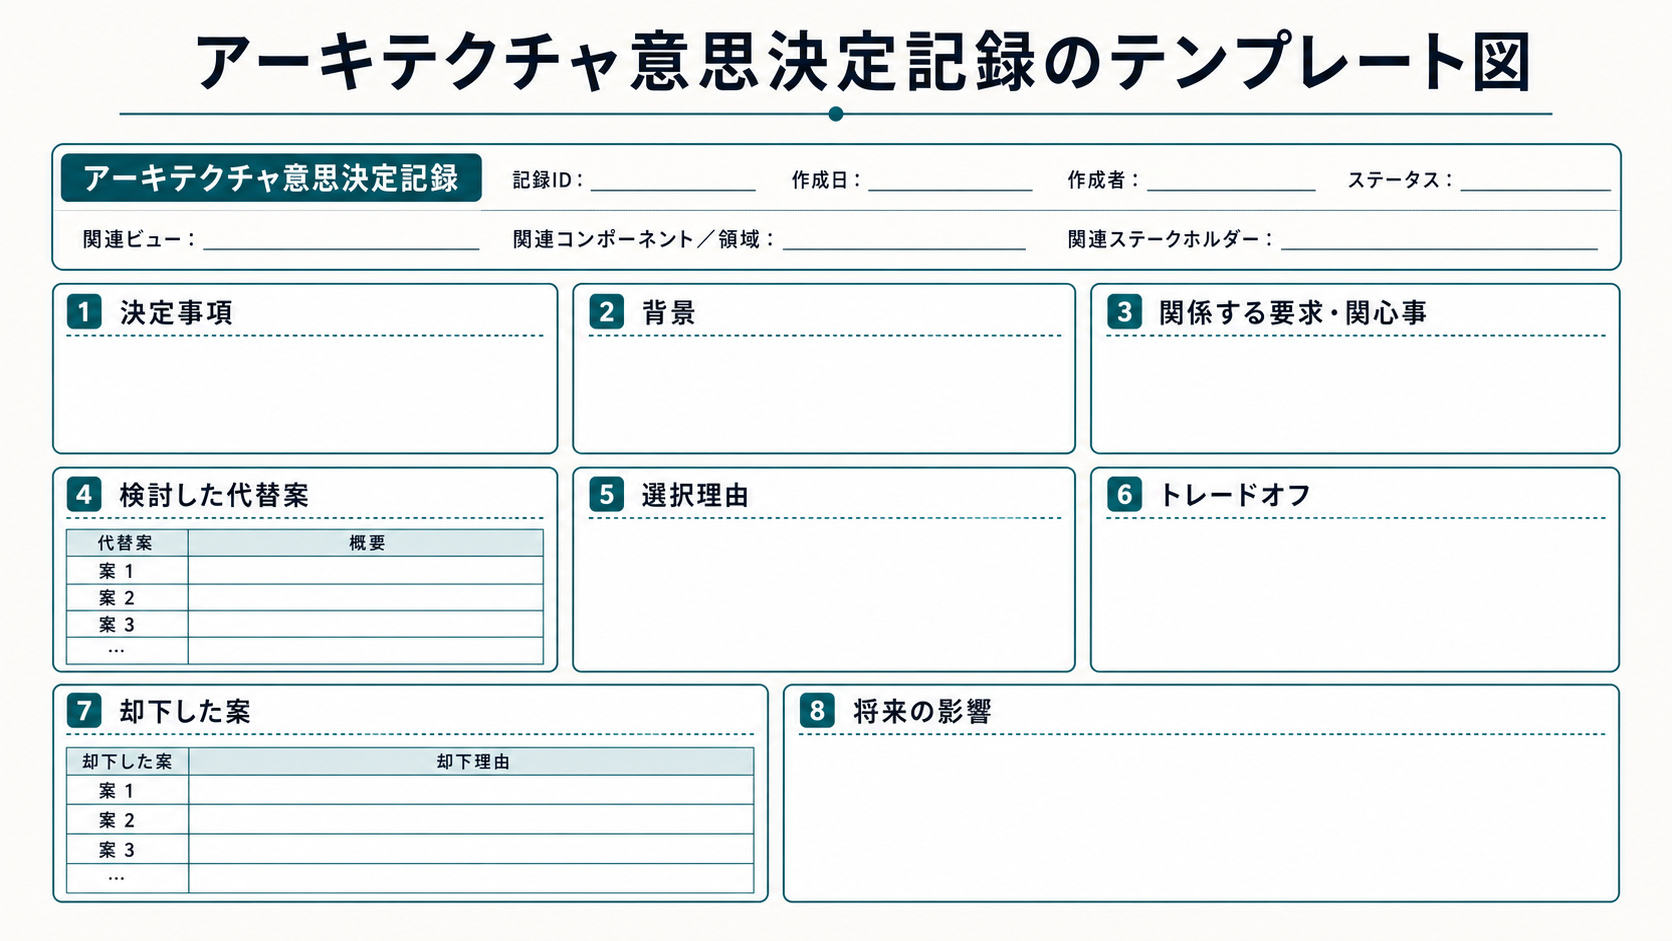
\includegraphics[width=0.96\linewidth]{assets/generated_figures/ch02/fig-ch02-06.png}}{\fbox{\parbox[c][48mm][c]{0.9\linewidth}{\centering 画像生成待ち\\アーキテクチャ意思決定記録のテンプレート図}}}
\caption{アーキテクチャ意思決定記録のテンプレート図}
\label{fig:ch02-06}
\end{figure}
